\documentclass[a4paper,12pt,final]{article}
\usepackage{graphicx}
\usepackage{multicol}					
\setlength{\multicolsep}{0pt}
\title{
\begin{center}
  	
\includegraphics[scale=0.3]{101Logo.png} 
  \end{center}
  \textbf{\\}
CSIR - Distributed Application Manager\\
Project Management Document\\
}
\author{101 Solutions}

\begin{document}
\maketitle
\begin{center}
Version 0.9
\end{center}
\textbf{\\}
\textbf{\\}
\textbf{\\}
\textbf{\\}
\textbf{\\}
\textbf{\\}
\begin{center}
\begin{tabular}{|l|l|}
\hline
Francois Germishuizen & 11093618\\
\hline
Jaco Swanepoel & 11016354\\
\hline
Henko van Koesveld & 11009315\\
\hline
\end{tabular}
\end{center}
\thispagestyle{empty}
\newpage
\thispagestyle{empty}
\textbf{\large{Change Log}}
\vspace{6pt}\newline
\begin{tabular}{|l|l|l|l|}
\hline
\textbf{Date} & \textbf{Version} & \textbf{Description} & \textbf{Done by}\\
\hline
12 Sept & Version 0.1 & Document Created & Jaco\\
\hline
12 Sept & Version 0.2 & Added member profiles & 101Solutions\\
\hline
12 Sept & Version 0.3 & Added burndown chart & Jaco\\
\hline
12 Sept & Version 0.4 & Added issue management content & Henko\\
\hline
12 Sept & Version 0.5 & Outstanding tasks / risks & Henko\\
\hline
12 Sept & Version 0.6 & Additions to  software development process & Henko\\
\hline
13 Sept & Version 0.7 & Grammar check & Jaco\\
\hline
24 Oktober & Version 0.8 & Updated new burndown chart & Jaco\\
\hline
24 Oktober & Version 0.9 & Additions to document & Henko\\
\hline
\end{tabular}
\newpage
\tableofcontents
\thispagestyle{empty}
\newpage

\pagenumbering{arabic}
\section{Overview}
\subsection{Background}
The CSIR is actively developing a distributed simulation framework that ties
in with various other real systems and is used to exchange information
between them. The client has a number of configurations of this system
depending on the requirements of the client which can involve various
external applications as well.\\
\textbf{\\}
One of the issues the client has is to quickly distribute the latest build or
configuration files of their software over various computers that are needed
for an experiment. In some cases the same computers may be used for other
experiments which mean each of the computers may need to have various
builds and configuration options.\\
\textbf{\\}
Another issue they experience is the running, stopping and restarting of
the complete simulation. During a simulation it may be determined that
certain configuration options may need to be changed and distributed to the
affected machines, in which case either all or some components will need to
be restarted which can become tedious and time consuming.
\subsection{Business opportunity}
The goal of our project is to develop an application which is able to maintain
various build versions of the simulation framework and distribute these builds
to certain designated machines that may be required for an experiment. The
application will monitor system statistics of the various machines attached
to an experiment and will have the ability to execute applications on those
machines which will have different configuration options.\\
\textbf{\\}
The application will consist of a master and slave component where the
master is used to control the distribution of slaves. From the master one will
be able to start an experiment which will run the relevant applications on all
the necessary machines.



\newpage
\section{Software development process}
The software development process that we have opted for is an
agile based approach by which we are able to continually improve 
on the current state that the project is in. We strive to always have
a working project in version control(Git) to ensure that if we need to
show our progress, it is there.\\
\textbf{\\}
Our framework for project management that we are using is scrum methodology 
which we use to ensure that our project stays on track. Our sprints take
place on a week to week basis where we meet in the beginning of each week
or during the weekend. During these meetings we discuss the current
progress and what is to be done for the next week. Daily we
also have small meetings if neccessary where we discuss project related work and problems that occur.\\
\textbf{\\}
Another reason for choosing the agile approach is the continous change that it
allows us to incoroporate. This allows us to change when the client changes the
requirements and allows us to more easily adapt to that change.

\newpage
\section{Member Profiles}
\subsection{Francois Germishuizen}
\begin{center}
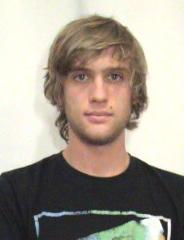
\includegraphics[width=3cm]{Francois.jpg}
\end{center}
\textbf{Skills:}
\begin{itemize}
\item General
\begin{itemize}
\item Web Development
\item Database Design
\item Software Design
\item Particular interest in computer networks
\end{itemize}
\item Programming and Markup Languages
\begin{itemize}
\begin{multicols}{2}
\item C++
	\item C\#
	\item Java
	\item PHP
	\item MySQL
    \item Microsoft SQL Server
	\item XML
    \item XSLT
    \item HTML
    \item CSS
	\item Javascript
    \item Qt, learn't during project
\end{multicols}
\end{itemize}
\end{itemize}
\textbf{Responsibilities:}
\begin{itemize}
\item Continuous work on the main project
\end{itemize}



\newpage
\subsection{Jaco Swanepoel}
\begin{center}
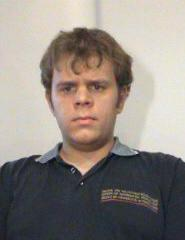
\includegraphics[width=3cm]{jaco.jpg}
\end{center}
\textbf{Skills:}
\begin{itemize}
\item General
\begin{itemize}
\item Organized
	\item Detail Oriented
	\item Reliable
	\item Work well under pressure
\end{itemize}
\item Programming Languages
\begin{itemize}
\begin{multicols}{2}
\item C
    \item C++
	\item C\#
	\item Java
    \item Basic Ruby
    \item Delphi
    \item Qt, learn't during project
\end{multicols}
\end{itemize}
\item Web development
\begin{itemize}
\begin{multicols}{2}
	\item HTML5
	\item CSS3
	\item JavaScript
	\item JSON
    \item JQuery
    \item Microsoft Sql Server
    \item MySql
    \item PHP
    \item XML
    \item Basic XSL
    \item Basic DTD and Schema
\end{multicols}
\end{itemize}
\end{itemize}
\textbf{Responsibilities:}
\begin{itemize}
\item Continuous work on the main project
\item Admin and client communications
\end{itemize}


\newpage
\subsection{Henko van Koesveld}
\begin{center}
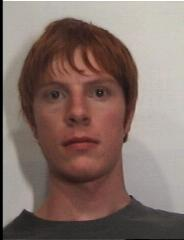
\includegraphics[width=3cm]{Henko.jpeg}
\end{center}
\textbf{Skills:}
\begin{itemize}
\item General
\begin{itemize}
	\item Database Design and Setup as well as normalization
	\item Software design with a focus on extensibility and maintenance
	\item Experience in various programming languages
	\item Hard working, dedicated
	\item Patience in solving problems
	\item Well experienced with HTML5 Web development
	\item Past experience with Qt framework
\end{itemize}
\item Programming and Markup Languages
\begin{itemize}
\begin{multicols}{2}
	\item C++
	\item Qt
	\item C\#
	\item Java
	\item PHP
	\item MySQL, Microsoft SQL Server
	\item XML, XSLT, HTML, CSS, JSON, JQuery, Javascript
	\item Knowledge in Assembly, Ruby and Delphi
\end{multicols}
\end{itemize}
\end{itemize}
\textbf{Responsibilities:}
\begin{itemize}
\item Continuous work on the main project
\item Keep the team updated on some work that needs to be done
\end{itemize}


\newpage

\section{Project management tools}
\subsection{Qt Framework}
The Qt framework allowed us to handle multiple project management issues. This allowed us to manage the project files much more easily if we had to do that ourself. A good example is the makefile which we did not have to write on our own since the qmake is able to do that for us.

\subsection{File management}
All files was handled by making use of a .pro file which is used in QT to use for building process. The files names are inside the .pro file under the respective title such as headers, source files, etc.

\subsection{QT Creator}
QT creator 2.7 allows one to make use of various version control systems including github.


\subsection{Code quality}
The Qt project management allows one to make use of a template which describes some of the code consistency that must be followed in order to keep the coding style similar. We followed the same coding style throughout the project and also documented thoroughly.

\subsection{Version control system}
We made use of GitHub as our version control system and that allowed us to ensure that there exist a single repository with our project. We always ensured that the project that is currently there is able to run.

\section{Issue Management}
This section describes how we report issues with the current software as it is and how we will go about resolving those issues. 
\subsection{Priorities}
Each issue is assigned a priority whereby it is handled as such. 
\subsection{Tools}
We first opted for a document based bug tracking software. We then later changed bugtracking to an online available form. We have changed to making use of FogBugz which allows us to have a 45 day free period where we can file any.\\
\textbf{\\}
FogBugz allows us to set certain tasks that are to be done. One can set the priority of the task such as, scale from 4 to 6 for "Fix if time" where one can be able to fix it if there is time, and a scale of 1 to 3 for "Must Fix" where it must be fixed. The last one is 7 which means that it does not have to be fixed.\\
\textbf{\\}
This website is not however only meant for the use in errors in code, but also things that must be changed and work that needs to be done. Work such as features that is still misssing, or even work that is still to be done. Other features that are used are the dates where we set out dates in which we believe that item should be done and handled.\\
\textbf{\\}
Our link to the bug tracking and handling site is appman.fogbugz.com. That is where the majority of bug tracking and job tasks are tracked and handled. The goals we set out are prioritized according to how important that is. Thus we can easily see what is more important than other tasks. 

\newpage
\section{Burndown Chart}
\begin{center}
\textbf{Burndown chart as at Friday 6 September, iteration 3 demo\\}
\end{center}
\begin{center}
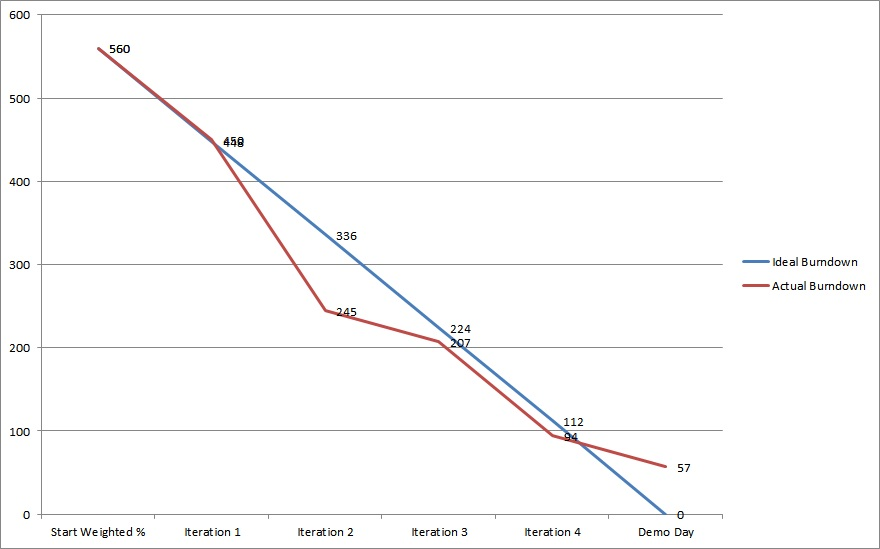
\includegraphics[scale=0.7]{Burndown.jpg}
\end{center}




\section{Outstanding tasks / risks}
We are currently still working on the following things:
\begin{itemize}
\item Delete a simulation
\item Edit simulation information
\end{itemize}
\end{document}